\let\negmedspace\undefined
\let\negthickspace\undefined
\documentclass[journal]{IEEEtran}
\usepackage[a5paper, margin=10mm, onecolumn]{geometry}
%\usepackage{lmodern} % Ensure lmodern is loaded for pdflatex
\usepackage{tfrupee} % Include tfrupee package

\setlength{\headheight}{1cm} % Set the height of the header box
\setlength{\headsep}{0mm}     % Set the distance between the header box and the top of the text

\usepackage{gvv-book}
\usepackage{gvv}
\usepackage{cite}
\usepackage{amsmath,amssymb,amsfonts,amsthm}
\usepackage{algorithmic}
\usepackage{graphicx}
\usepackage{textcomp}
\usepackage{xcolor}
\usepackage{txfonts}
\usepackage{listings}
\usepackage{enumitem}
\usepackage{mathtools}
\usepackage{gensymb}
\usepackage{comment}
\usepackage[breaklinks=true]{hyperref}
\usepackage{tkz-euclide} 
\usepackage{listings}
% \usepackage{gvv}                               

\def\inputGnumericTable{}                      
\usepackage[latin1]{inputenc}                    
\usepackage{color}                              
\usepackage{array}                             
\usepackage{longtable}                          
\usepackage{calc}                               
\usepackage{multirow}                           
\usepackage{hhline}                            
\usepackage{ifthen}                          
\usepackage{lscape}
\begin{document}

\bibliographystyle{IEEEtran}
\vspace{3cm}

\title{4.13.93}
\author{AI25BTECH11024 - Pratyush Panda
}
\maketitle
% \newpage
% \bigskip
{\let\newpage\relax\maketitle}

\renewcommand{\thefigure}{\theenumi}
\renewcommand{\thetable}{\theenumi}
\setlength{\intextsep}{10pt} % Space between text and floats


\numberwithin{equation}{enumi}
\numberwithin{figure}{enumi}
\renewcommand{\thetable}{\theenumi}

\textbf{Question: } \\
Let $\Vec{P}$ be the image of the point $\brak{3,1,7}$ with respect to the plane $x-y+z=3$. Then the equation of the plane passing through $\Vec{P}$ and containing the straight line $\frac{x}{1}=\frac{y}{2}=\frac{z}{1}$ is
\begin{enumerate}
\item $x+y-3z=0$
\item $x-4y+7z=0$
\item $x+3z=0$
\item $2x-y=0$
\end{enumerate}
\vspace{0.7cm}

\textbf{Solution: } \\
Let the vector $\Vec{A}=\myvec{3 \\ 1 \\ 7}$. \\

The given plane can be written as;
\begin{align}
\Vec{n_1}^T\Vec{X}=3 \hspace{1cm} where, \, \Vec{n_1}=\myvec{1 \\ -1 \\ 1}
\end{align}

And the line has the direction vector $\Vec{b}$=$\myvec{1 \\ 2 \\ 1}$

Now, the image of point $\Vec{A}$ with respect to the plane can be found out by the formula;
\begin{align}
\Vec{P}=\Vec{A}-\frac{2\brak{\Vec{n}^T\Vec{A}-3}}{||\Vec{n}||}\Vec{n}
\end{align}

From putting the values in the formula, we get the point $\Vec{P}$ to be $\myvec{-1 \\ 5 \\ 3}$

Let the equation of the required plane be $\Vec{X}^T\Vec{n}=0$ since the plane contains the line and the line passes through the origin. \\

From the given constraints we can get the following equations;
\begin{align}
\Vec{P}^T\Vec{n}=0 && \Vec{b}^T\Vec{n}=0
\end{align}

If we combine the two equations we get;
\begin{align}
\myvec{P & b}^T\Vec{n}=\myvec{0 \\ 0}
\end{align}

On solving this equation we get $\Vec{n}=n.\myvec{1 \\ -4 \\ 7}$. The parameter can be taken as 1. \\

Thus, the equation of the required plane is $\myvec{1 \\ -4 \\ 7}^T\Vec{X}=0$ or $x-4y+7z=0$.

\begin{figure}[H]
\centering
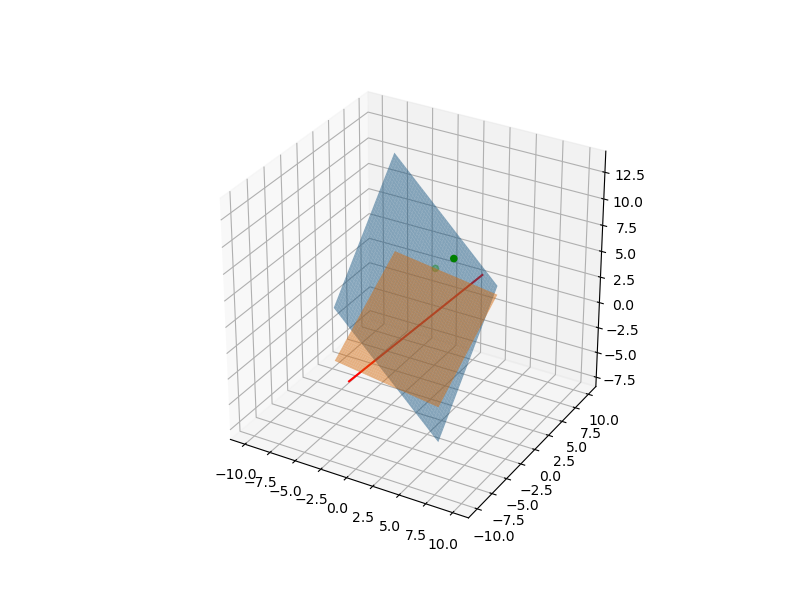
\includegraphics[width=0.8\columnwidth]{figs/img.png}
\caption*{}
\end{figure}

\end{document}
